%% pairwise_genome_alignment.tex
%% Author: Leighton Pritchard
%% Copyright: James Hutton Institute
%% Pairwise genome alignment approaches

%
\begin{frame}
  \frametitle{Pairwise genome alignments}
  \textcolor{olive}{Genome sequence data gives us much more detail and power} \\
  Pairwise comparisons require alignment of similar regions.
  \begin{center}
    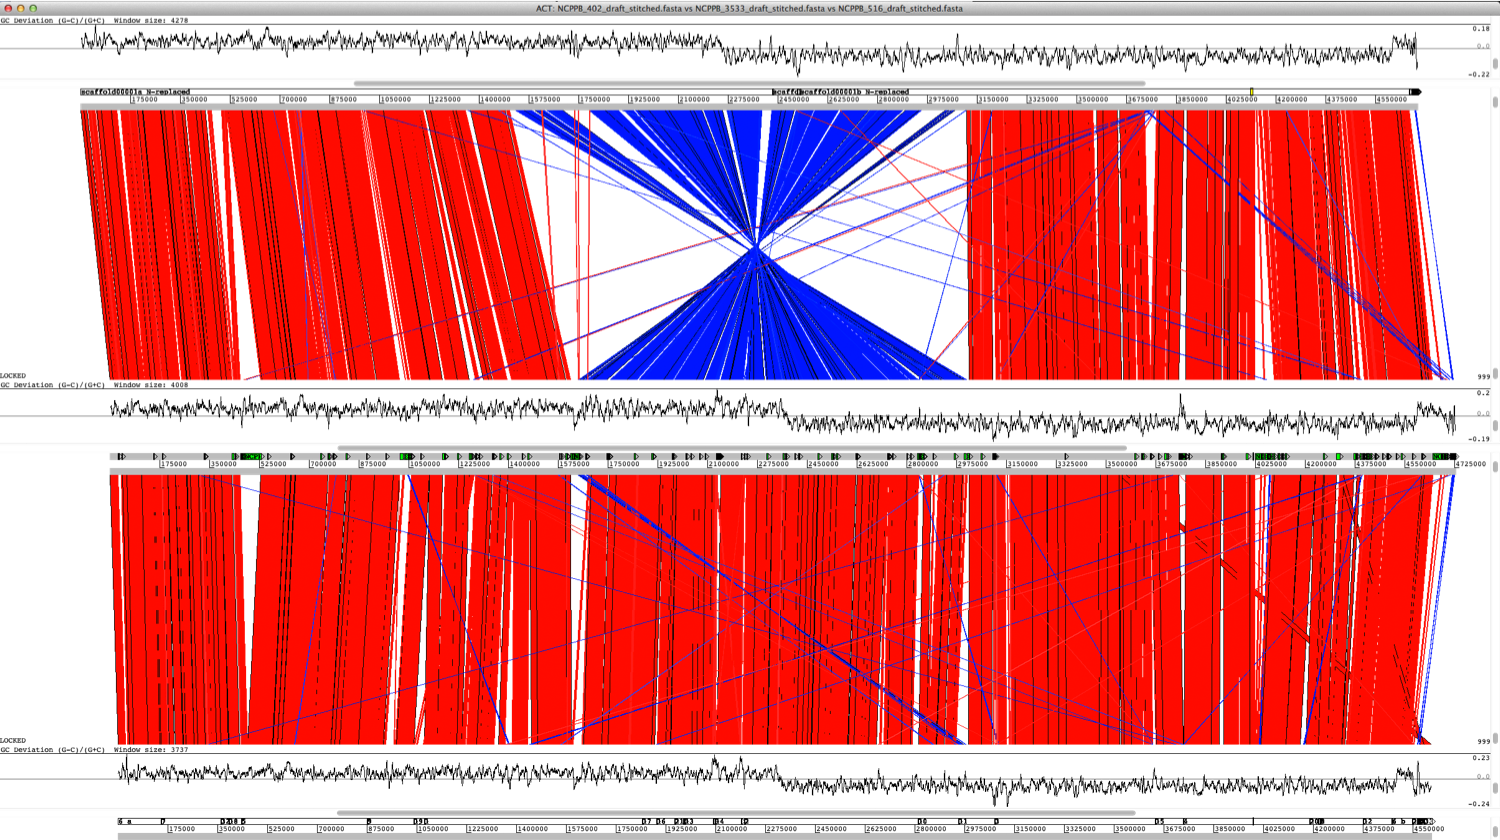
\includegraphics[width=\textwidth]{images/pairwise_genome_alignment}
  \end{center}  
\end{frame}

%
\begin{frame}
  \frametitle{Pairwise genome alignments}
  \textcolor{hutton_green}{Which genomes should you align (or not bother with)?} \\
  \textcolor{RawSienna}{For reasonable analysis, genomes should}:
  \begin{itemize}
    \item derive from a sufficiently \textcolor{red}{recent} common ancestor, so that \textcolor{hutton_purple}{homologous regions can be identified}
    \item derive from a sufficiently \textcolor{red}{distant} common ancestor, so that \textcolor{hutton_purple}{biologically meaningful changes are likely to be found}
  \end{itemize}
\end{frame}

%
\begin{frame}
  \frametitle{Alignment algorithms/programs}
  \textcolor{hutton_green}{I assume you're familiar with BLAST} \\
  (but, if not, see \url{supporting_information} subdirectory) \\~\\
  \textcolor{RawSienna}{Na\"{i}ve alignment algorithms are not appropriate}:
  \begin{itemize}
    \item Needleman-Wunsch: optimal global alignment
    \item Smith-Waterman: optimal local alignment
  \end{itemize}
  \textcolor{hutton_blue}{Cannot handle rearrangement} \\
  \textcolor{hutton_purple}{Computationally expensive}  
\end{frame}

%
\begin{frame}
  \frametitle{Alignment algorithms/programs}
  \textcolor{hutton_green}{Many whole-genome alignment algorithms proposed} \\
  Handle genome-scale evolutionary processes, scalable \\~\\
  \begin{itemize}
    \item \href{http://www.bx.psu.edu/~rsharris/lastz/}{LASTZ (http://www.bx.psu.edu/\~rsharris/lastz/)}
    \item \href{http://genome.ucsc.edu/goldenPath/help/blatSpec.html}{\textcolor{hutton_blue}{\textbf{BLAT} (http://genome.ucsc.edu/goldenPath)}}
    \item \href{http://mugsy.sourceforge.net/}{Mugsy (http://mugsy.sourceforge.net/)}
    \item \href{http://www.ncbi.nlm.nih.gov/blast/html/megablast.html}{\textcolor{red}{\textbf{megaBLAST} (http://www.ncbi.nlm.nih.gov/blast/)}}
    \item \href{http://mummer.sourceforge.net/}{\textcolor{red}{\textbf{MUMmer} (http://mummer.sourceforge.net/)}}
    \item \href{http://lagan.stanford.edu/lagan_web/index.shtml}{LAGAN (http://lagan.stanford.edu/lagan\_web/index.shtml)}
    \item WABA, etc?
  \end{itemize}
\end{frame}

%
\begin{frame}
  \frametitle{BLAT
  \footnote{\tiny{\href{http://dx.doi.org/10.1101/gr.229202
}{Kent (2002) \textit{Genome Res.} doi:10.1101/gr.229202
}}}
  }
  Broadly similar to BLAST \\~\\
  \textcolor{hutton_blue}{Main differences:}
  \begin{itemize}
    \item optimised to find \textcolor{hutton_purple}{only exact or near-exact matches} (speed)
    \item indexes the subject genome, and \textcolor{hutton_purple}{\textit{scans the query}}
    \item connects homologous match regions into a single alignment (BLAST reports separately)
    \item reports mRNA match intron-exon bounds exactly (BLAST tends to extend beyond bounds)
  \end{itemize}
  \textcolor{hutton_green}{\textbf{ADVANTAGES}: fast, exact exon bounds, UCSC integration}
  \textcolor{RawSienna}{\textbf{DISADVANTAGES}: less sensitive on remote/divergent sequences}
\end{frame}